\documentclass[12pt]{article}
\usepackage{tikz}

\usepackage{amsfonts, amsmath, amssymb}
\usepackage{systeme, mathtools}

\usetikzlibrary{positioning, arrows.meta, quotes} % 定位节点, 自定义箭头的连线, 给节点连线快速加文本标注
\usetikzlibrary{shapes, snakes} % 绘制流程图、UML 图, 绘制不规则曲线
\usetikzlibrary{bayesnet} % 加载贝叶斯网络专用库
\tikzset{>=latex} % 设置 TikZ 中所有箭头的默认样式为 latex 风格

\begin{document}
%% 基本曲线
\begin{tikzpicture}
    % 绘制矩形、圆形和曲线
    \draw [red] (0, 0) rectangle (1.5, 1);
    \draw [blue, ultra thick] (3, 0.5) circle [radius=0.5];
    \draw [green] (6, 0) arc [radius=1.5, start angle=45, end angle=100];
    % 绘制圆角的坐标系
    \draw [<->, rounded corners, thick, purple] (0, -2) -- (0, -4) -- (3, -4);
    % 绘制过渡曲线
    \draw [<-, thick] (5, -2) -- (5, -3.5);
    \draw [thick, red] (5, -3.5) to [out=270, in=180] (5.5, -4);
    \draw [->, thick] (5.5, -4) -- (8, -4);
    % 绘制 S 曲线
    \draw [<->, thick, blue] (0, -6) to [out=90, in=180] (1, -5) to [out=0, in=180] (3, -6) to [out=0, in=-90] (4, -5);
\end{tikzpicture}

\newpage
%% 根据函数绘制曲线
% 阶乘函数factorial(\x), 平方根sqrt(\x), 幂函数pow(\x,y), 指数函数exp(\x), 对数函数ln(\x), log10(\x), log2(\x), abs(\x), 取余函数mod(\x,y), 圆整函数round(\x), floor(\x), ceil(\x), sin(\x), cos(\x), tan(\x)等。(\x r)
% 常数:e=2.718281828, pi=3.141592654
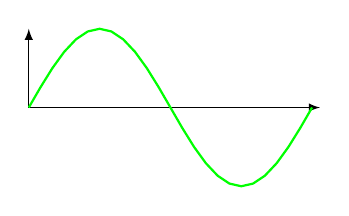
\begin{tikzpicture}[xscale=0.01, yscale=1]
    \draw [<->] (0, 1) -- (0, 0) -- (370, 0);
    \draw [green, thick, domain=0:360] plot (\x, {sin(\x)}); % domain表示自变量取值范围,默认角度; 数学表达式需要加{}
\end{tikzpicture}

% 组合基本函数
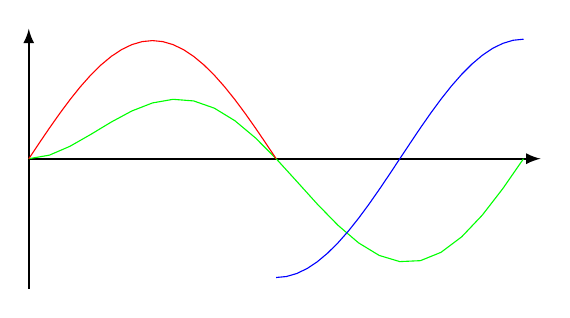
\begin{tikzpicture}[yscale=1.5]
    \draw [thick, ->] (0, 0) -- (6.5, 0);
    \draw [thick, ->] (0, -1.1) -- (0, 1.1);
    \draw [green, domain=0:2*pi] plot (\x, {sin(\x r) * ln(\x+1)/2}); % (\x r)表示弧度
    \draw [red, domain=0:pi] plot (\x, {sin(\x r)});
    \draw [blue, domain=pi:2*pi] plot (\x, {cos(\x r) * exp(\x/exp(2*pi))});
\end{tikzpicture}

%% 区域填充
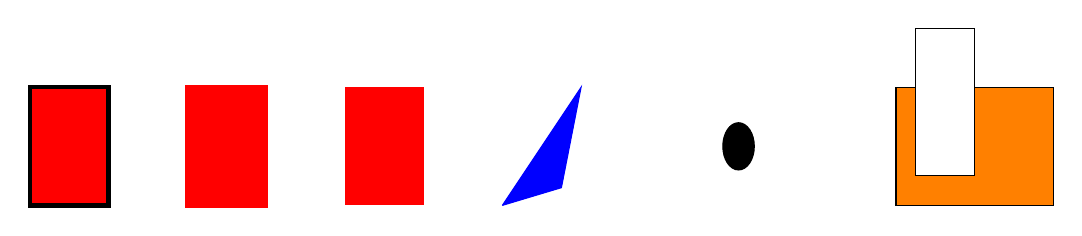
\begin{tikzpicture}[yscale=1.5]
    \draw [fill=red, ultra thick] (0, 0) rectangle (1, 1);
    \draw [fill=red, ultra thick, red] (2, 0) rectangle (3, 1); % 第二个red声明边框线的颜色
    \path [fill=red, ultra thick] (4, 0) rectangle (5, 1); % \path 替换 \draw 绘制无边框图形
    \draw [blue, fill=blue] (6, 0) -- (7, 1) -- (6.75, 0.15) -- (6, 0);
    \draw [fill] (9, 0.5) circle [radius=0.2]; % fill 默认填充黑色
    \draw [fill=orange] (11, 0) rectangle (13, 1);
    \draw [fill=white] (11.25, 0.25) rectangle (12, 1.5);
\end{tikzpicture}

\vspace{2cm}
%% 填写标签
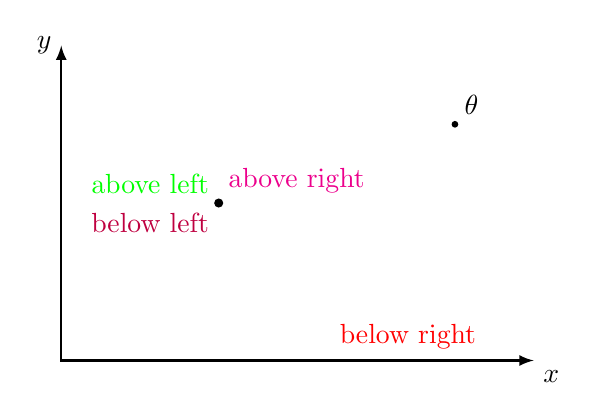
\begin{tikzpicture}[xscale=2, yscale=2]
    % 绘制坐标轴
    \draw [thick, <->] (0, 2) -- (0, 0) -- (3, 0);
    \draw [fill] (1, 1) circle [radius=0.025];
    \node [below right] at (3, 0) {$x$};
    \node [left] at (0, 2) {$y$};
    % 标注点 (1, 1)
    \node [below right=2, red] at (1, 1) {below right};
    \node [above left, green] at (1, 1) {above left};
    \node [below left, purple] at (1, 1) {below left};
    \node [above right, magenta] at (1, 1) {above right};
    % 插入数学符号 \theta
    \draw[fill] (2.5, 1.5) circle [radius=0.5pt];
    \node [above right] at (2.5, 1.5) {$\theta$};
\end{tikzpicture}

\newpage
%% 矩阵分解示意图
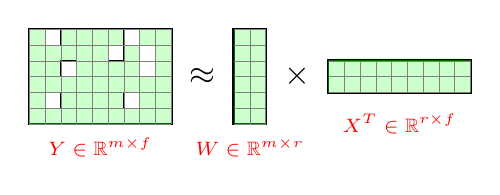
\begin{tikzpicture}
    \draw [very thick] (0, 0) rectangle (3.6/2, 2.4/2);
    \filldraw [fill=green!20!white, draw=green!40!black] (0, 0) rectangle (3.6/2, 2.4/2);
    \filldraw [fill=white] (0.4/2, 0.4/2) rectangle (0.8/2, 0.8/2);
    \filldraw [fill=white] (2.4/2, 0.4/2) rectangle (2.8/2, 0.8/2);
    \filldraw [fill=white] (0.8/2, 1.2/2) rectangle (1.2/2, 1.6/2);
    \filldraw [fill=white] (2.0/2, 1.6/2) rectangle (2.4/2, 2.0/2);
    \filldraw [fill=white] (0.4/2, 2.0/2) rectangle (0.8/2, 2.4/2);
    \filldraw [fill=white] (2.4/2, 2.0/2) rectangle (2.8/2, 2.4/2);
    \filldraw [fill=white] (2.8/2, 1.2/2) rectangle (3.2/2, 2.0/2);
    \draw [step=0.4/2, very thin, color=gray] (0, 0) grid (3.6/2, 2.4/2);
    \draw (1.8/2, -0.3) node {{\color{red} \scriptsize{$Y\in\mathbb{R}^{m \times f}$}}};
    
    \draw (4.4/2, 1.2/2) node {{\color{black}\large{$\approx$}}};

    \draw [very thick] (5.2/2, 0) rectangle (6.0/2, 2.4/2);
    \filldraw [fill=green!20!white, draw=green!40!black] (5.2/2, 0) rectangle (6.0/2, 2.4/2);
    \draw [step=0.4/2, very thin, color=gray] (5.2/2, 0) grid (6.0/2, 2.4/2);
    \draw (5.6/2, -0.3) node {{\color{red} \scriptsize{$W\in\mathbb{R}^{m \times r}$}}};

    \draw (6.8/2, 1.2/2) node {{\color{black}\large{$\times$}}};

    \draw [very thick] (7.6/2, 0.8/2) rectangle (11.2/2, 1.6/2);
    \filldraw [fill=green!20!white, draw=green!40!black] (7.6/2, 0.8/2) rectangle (11.2/2, 1.6/2);
    \draw [step=0.4/2, very thin, color=gray] (7.6/2, 0.8/2) grid (11.2/2, 1.6/2);
    \draw (9.4/2, 0) node {{\color{red} \scriptsize{$X^{T}\in\mathbb{R}^{r \times f}$}}};
\end{tikzpicture}


\end{document}
